\documentclass[11pt]{article}

\usepackage[utf8]{inputenc}
\usepackage[spanish]{babel}
\usepackage[vmargin=2.5cm,hmargin=2.5cm]{geometry}
\usepackage{enumerate}
\usepackage{algpseudocode}
\usepackage{graphics,graphicx,float} %para incluir imágenes y colocarlas
\usepackage{spverbatim}

\title{Práctica	1: Robótica \\
Entrega 2: Explorador basado en fronteras}

\author{ Elena María Gómez Ríos }


\begin{document}

\maketitle

\section{Análisis del problema}
La tarea principal de esta práctica es implementar un explorador basado en fronteras para que un robot pueda reconocer el mapa de su entorno. Para esta práctica hemos utilizado como base el código proporcionado por los profesores de prácticas de la asignatura llamado ``mi\_mapeo\_stage''.\\

Para realizar la práctica lo que hemos hecho ha sido realizar las tareas siguientes:
\begin{itemize}
	\item Girar 360º.
	\item Detectar la frontera.
	\item Seleccionar un punto de la frontera.
	\item Enviar el robot a ese punto objetivo.
	\item Adoptar una estrategia si no se alcanza el objetivo.
\end{itemize}


\section{Descripción de la solución planteada}

El problema se ha resuelto repitiendo las tareas anteriormente nombradas. Dichas tareas las he implementado en distintos métodos los cuales voy a explicarlos detalladamente a continuación.

\subsection{Girar 360º}
Este problema se ha resuelto en el método \texttt{gira360} el cual realiza 2 giros completos sobre sí mismo para así analizar el entorno del robot para poder tomar una mejor decisión a la hora de dirigirnos hacia la frontera.\\

Para implementarlo he utilizado la velocidad angular con la que gira el robot para así poder calcular el tiempo de giro de una vuelta completa. De este modo controlando el tiempo que gira el robot podemos hacer que de dos vueltas completas sobre sí mismo.\\

Una posible solución en pseudocódigo de esta idea es:

\begin{verbatim}
tiempo final = tiempo actual + tiempo velocidad angular * 2
mientras (tiempo actual < tiempo final)
    gira
\end{verbatim}


\subsection{Detectar la frontera}
En este caso el problema se ha resuelto modificando el método \texttt{getmapCallBack} y con el método \texttt{labelFrontierNodes}.\\

La modificación realizada en el método \texttt{getmapCallBack} ha sido incluir una llamada al método \texttt{rellenaObstaculos} el cual modifica el mapa theGlobalCm entorno a un metro cuadrado de una celda obstáculo. Para ello realizo dos bucles que recorren una matriz al rededor del obstáculo marcando las casillas como 100 (obstáculo) y utilizando una matriz de variable booleana para controlar que esas modificaciones no se eliminen en siguientes iteraciones del bucle principal del método \texttt{getmapCallBack}.\\

El método \texttt{labelFrontierNodes} inserta en una lista llamada ``frontera'' los puntos del mapa conocido que tienen algún vecino desconocido. Para ello se utiliza el método \texttt{someNeighbourIsUnknown} que devuelve si una celda tiene un vecino desconocido. Por lo tanto este método recorre la matriz cmGlobal completa y cuando la celda sea igual a 0 (conocida) y exista un vecino desconocido para dicha celda se guardará el valor de la celda en la lista ``frontera''. Para evitar errores he utilizado el método eraseFrontier pasandole como argumento la posición del robot para así eliminar de la frontera los puntos situados debajo del robot. La lista frontera se limpia cada vez que se llama a este método.

\subsection{Seleccionar un punto de la frontera}
El problema está resuelto en el método \texttt{selectNode} con el que se selecciona el nodo de menor distancia entre dicho nodo y el robot que pertenezca a la lista de nodos guardados en ``frontera''. Como en ésta lista no se guardaban los nodos a una distancia de dos metros de la posición del robot evitaremos el problema de que el punto objetivo quede debajo del robot.

\subsection{Enviar el robot a ese punto objetivo}
Para enviar el robot al punto objetivo hemos utilizado el código de la sesión 5 de prácticas, simplemente cambiamos las variables x e y del goal a las variables de nuestro nodo objetivo.

\subsection{Adoptar una estrategia si no se alcanza el objetivo}
La estrategia a seguir si no se alcanza el objetivo es seleccionar el siguiente nodo más cercano.

\section{Análisis}
La ejecución me ha tardado unos 8,40 minutos en el mapa corridor que ha explorado al completo el mapa y la ejecución del mapa willow que no ha llegado a terminar porque se quedaba bloqueado después de una colisión cuando llevaba unos 30 minutos.\\

Las capturas de los mapas descubiertos son las siguientes:

\begin{figure}[H] 
	\centering
	
\includegraphics[width=15cm]{img/ejecucion1.png}
	\caption{Ejecución en el mapa corridor.}
\end{figure}

\begin{figure}[H] 
	\centering
	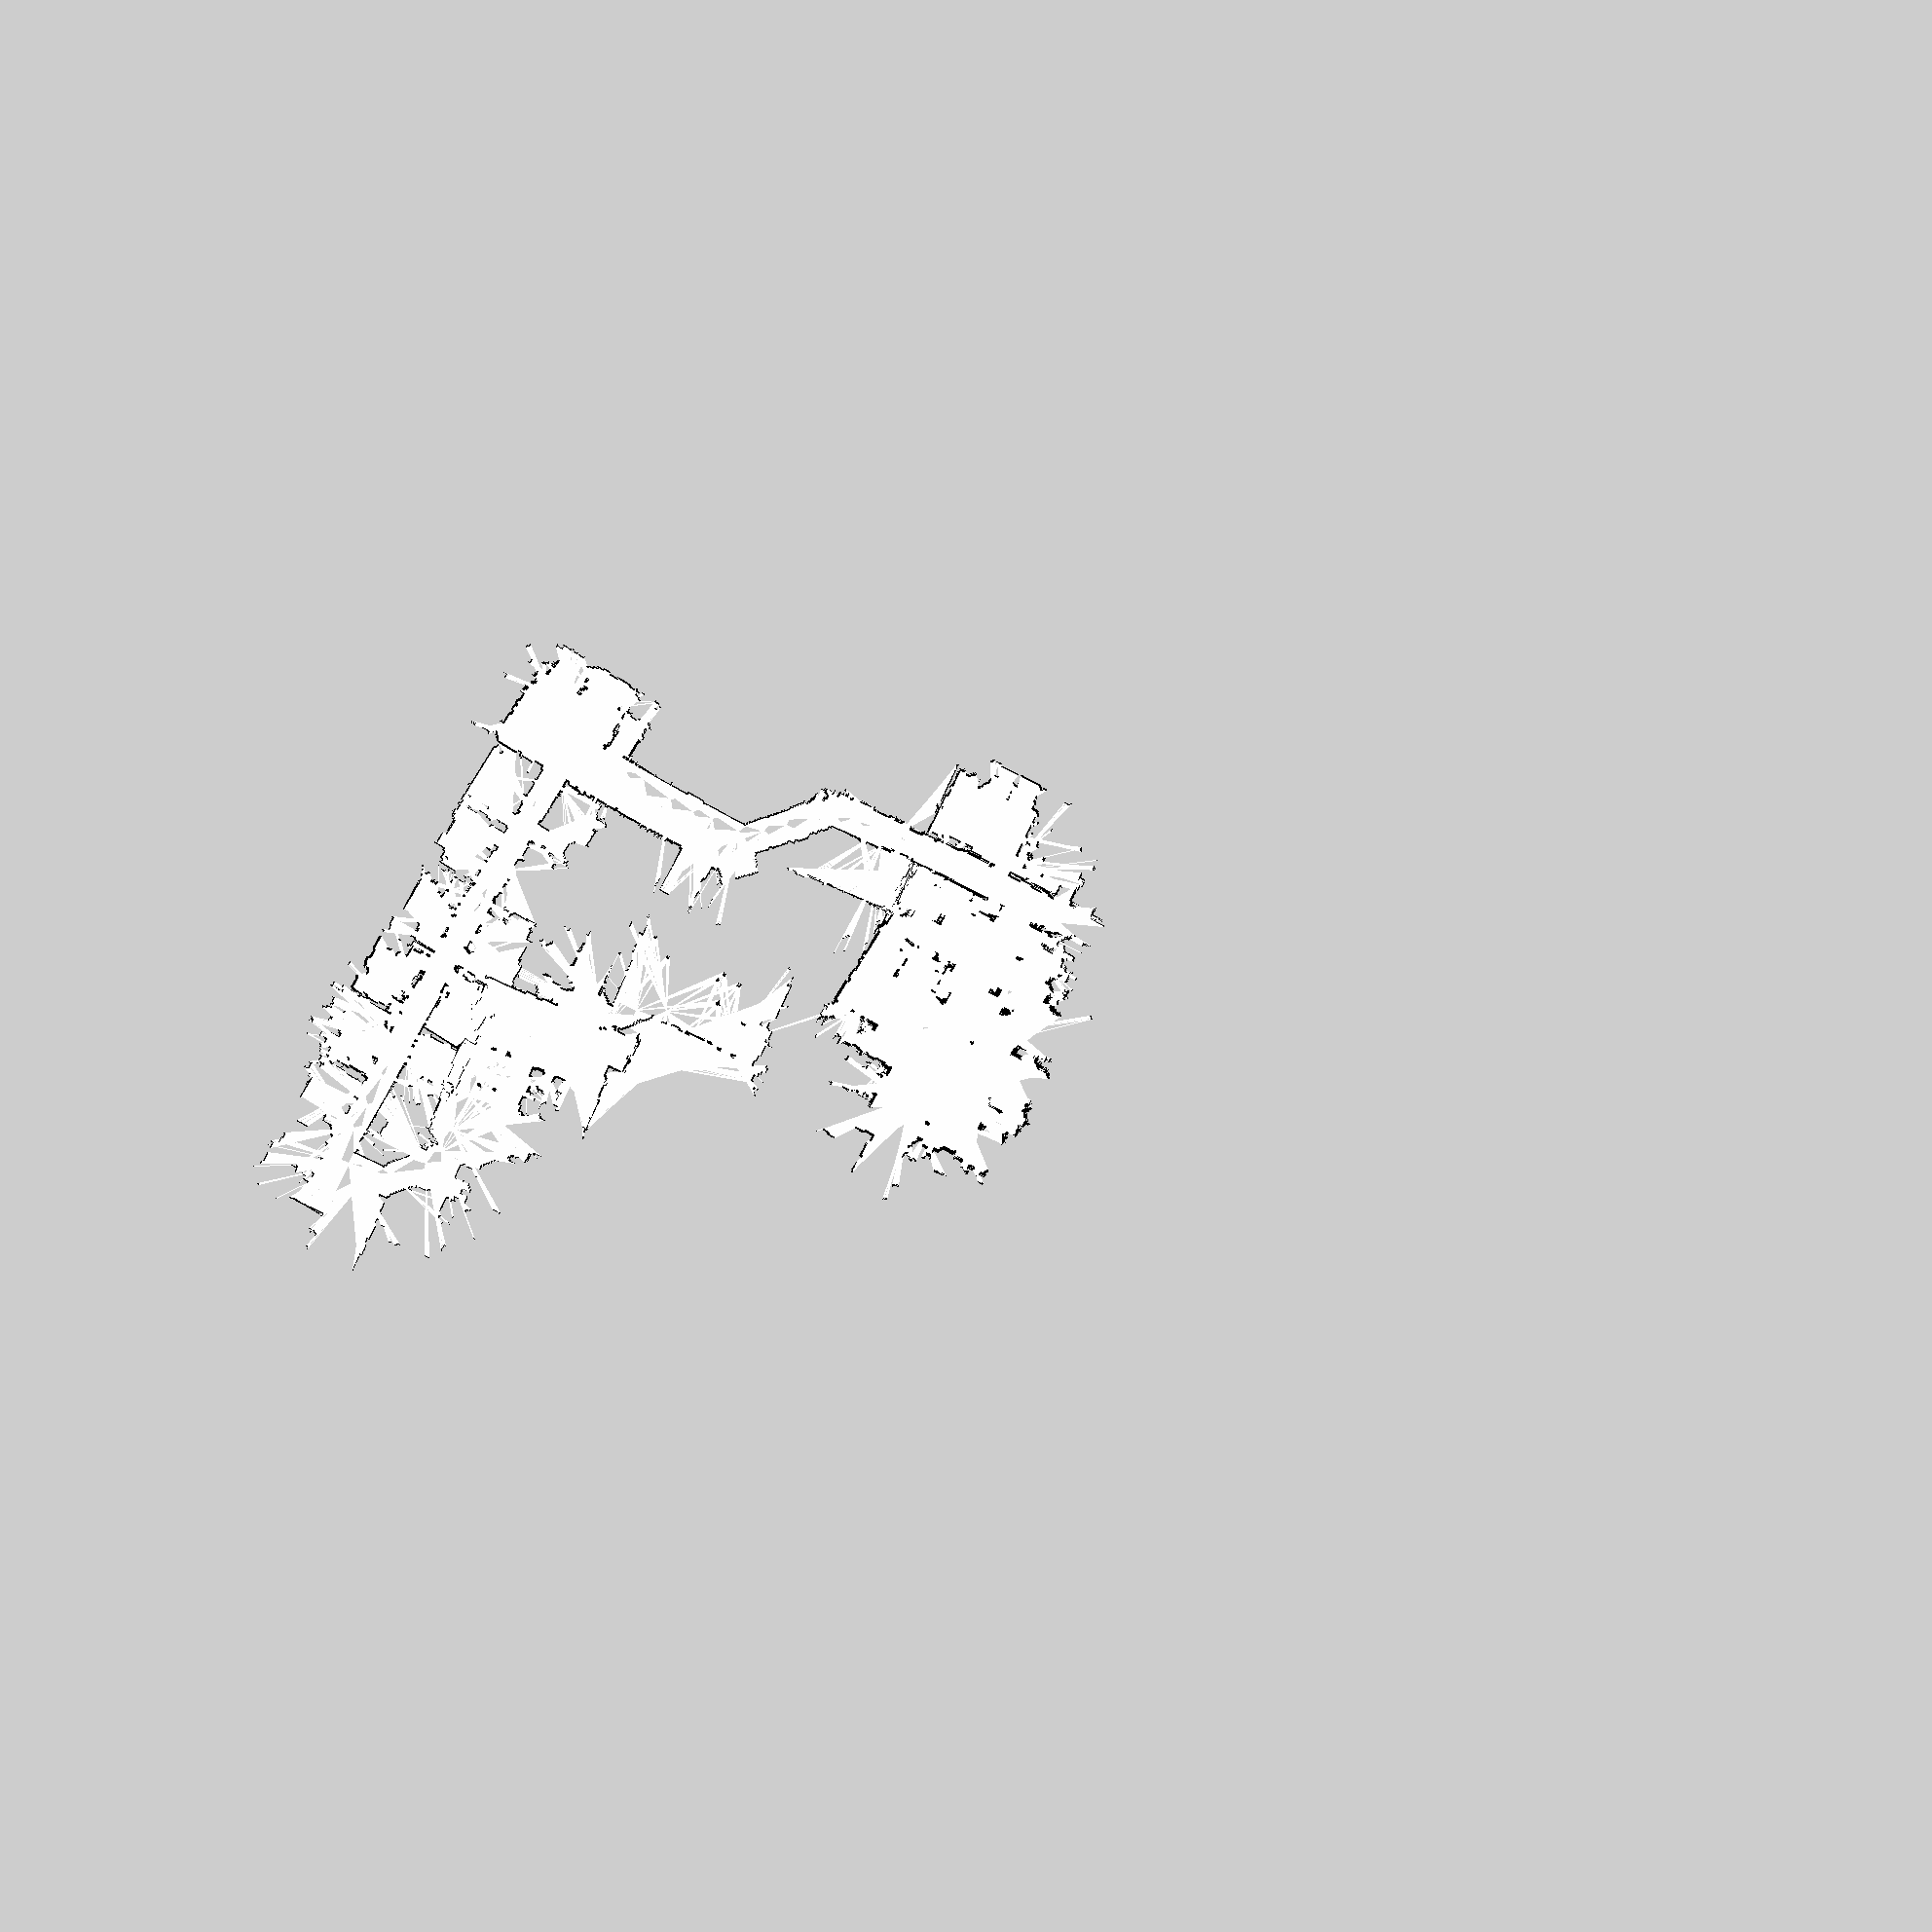
\includegraphics[width=15cm]{img/ejecucion2.png}
	\caption{Ejecución en el mapa willow.}
\end{figure}


\end{document}